% PREAMBLE
%%%%%%%%%%%%%%%%%%%%%%%%%%%%%%%%%%%%%%%%%%%%%%%%%%%%%%%%%%%%%%%%%%%%%%%%%%%%%%%%%%%%%%%%%%%%%%%%%%%%%%%%
%%%%%%%%%%%%%%%%%%%%%%%%%%%%%%%%%%%%%%%%%%%%%%%%%%%%%%%%%%%%%%%%%%%%%%%%%%%%%%%%%%%%%%%%%%%%%%%%%%%%%%%%
\documentclass[10pt]{article}
\usepackage{geometry}                	% See geometry.pdf to learn the layout options. There are lots.
\geometry{top=1.0in, bottom=1.0in, left=1.0in, right=1.0in}                   	% ... or a4paper or a5paper or ...
%\geometry{landscape}                	% Activate for for rotated page geometry
\usepackage{fancyhdr} 			% This should be set AFTER setting up the page geometry
\pagestyle{fancy} 				% options: empty , plain , fancy
\renewcommand{\headrulewidth}{0pt} % customise the layout...
\lhead{}\chead{}\rhead{}
\lfoot{}\cfoot{\thepage}\rfoot{}
%\usepackage[parfill]{parskip}   	   	% Activate to begin paragraphs with an empty line rather than an indent
\usepackage{graphicx}
\usepackage{amssymb}
\usepackage{epstopdf}
\usepackage{booktabs} 			% for much better looking tables
\usepackage{array} 				% for better arrays (eg matrices) in maths
\usepackage{paralist} 			% very flexible & customisable lists (eg. enumerate/itemize, etc.)
\usepackage{verbatim}			% adds environment for commenting out blocks of text & for better verbatim
\usepackage{subfigure} 			% make it possible to include more than one captioned figure/table in a single float
\usepackage{algorithmic}
\DeclareGraphicsRule{.tif}{png}{.png}{`convert #1 `dirname #1`/`basename #1 .tif`.png}
\usepackage{sectsty}
%\allsectionsfont{\sffamily\mdseries\upshape} 	% (See the fntguide.pdf for font help)
%\usepackage[utf8]{inputenc} 		% Any characters can be typed directly from the keyboard, eg éçñ
%\usepackage{textcomp} 		% provide lots of new symbols
\usepackage{graphicx}  			% Add graphics capabilities
\usepackage{epstopdf} 			% to include .eps graphics files with pdfLaTeX
\usepackage{flafter}  			% Don't place floats before their definition
\usepackage{amsmath,amssymb} 	% Better maths support & more symbols
\usepackage{bm}  				% Define \bm{} to use bold math fonts
\usepackage{memhfixc}  			% remove conflict between the memoir class & hyperref
%\usepackage{pdfsync}  			% enable tex source and pdf output syncronicity
\usepackage[pdftex,bookmarks,colorlinks,breaklinks]{hyperref}  % PDF hyperlinks, with coloured links
\hypersetup{linkcolor=black,citecolor=black,filecolor=black,urlcolor=black} % black links, for printed output
\usepackage{cite}
\usepackage{mathtools}
\usepackage{subfigure}			% for putting figures "side-by-side"
%\usepackage{sidecap}			% sidecaption figures
\usepackage{wrapfig}
\usepackage{caption}
\usepackage{multicol}

%\makeatletter
%\newenvironment{tablehere}
  %{\def\@captype{table}}
  %{}

%\newenvironment{figurehere}
 % {\def\@captype{figure}}
 % {}
%\makeatother


% Title Page
\title{\textbf{CBEMD}: Parallelized Molecular Dynamics in Various Thermodynamic Ensembles}
\author{Carmeline J. Dsilva, George A. Khoury, Nathan A. Mahynski,   \\
Junyoung Park, Arun Prabhu, and Francesco Ricci}
\date{}

\begin{document}
\maketitle
\begin{figure}[htbp]
   \centering
   
\includegraphics[width=2.5in]{princeton.jpg}
\end{figure}
\thispagestyle{empty}
\newpage
\setcounter{page}{1}
\pagenumbering{arabic}
\newpage

\section{Introduction}
We proposed to develop a software package to perform parallelized molecular dynamics (MD) for several different thermodynamic ensembles.
%
Molecular dynamics is a technique commonly used to simulate atomic/molecular motions on a microscopic level from which macroscopic properties can be calculated.
%
Properties such as diffusion coefficients, specific heats, and chemical potentials, which are often difficult or impossible to measure in experiment, are commonly available in MD.
%
%For instance, it has been commonly used to quantitatively measure the folding rate and stability of proteins, diffusivities of atoms and molecules in solution, viscosities, and other thermodynamic measurements at temperature or pressure extremes that are higher and lower than are experimentally convenient.
% 
This list is clearly non-exhaustive.
%
Because of the myriad of properties that can be calculated, MD has applications in such fields as material science, pharmaceutical design, cellular biology, thermodynamics, and fluid mechanics.
%
Due to its relative simplicity and its ability to be massively parallelized, MD is a common but powerful tool for many scientists and engineers today.

\section{Background on Molecular Dynamics}
MD first initializes a system of particles, with positions and often velocities.
%
If no initial velocities are assigned, they can be computed, but positions are required.
%
Given an interaction potential $V (\overrightarrow{r})$ between different types of particles, MD integrates Newton's equation of motion, $\overrightarrow{F}=m\overrightarrow{a}$, forward in time.
%
Figure~\ref{fig: workflow} shows the flow of the program schematically, which follows well defined steps:

\begin{wrapfigure}{l}{0.5\textwidth}
\vspace{-20pt}
	\begin{center}	 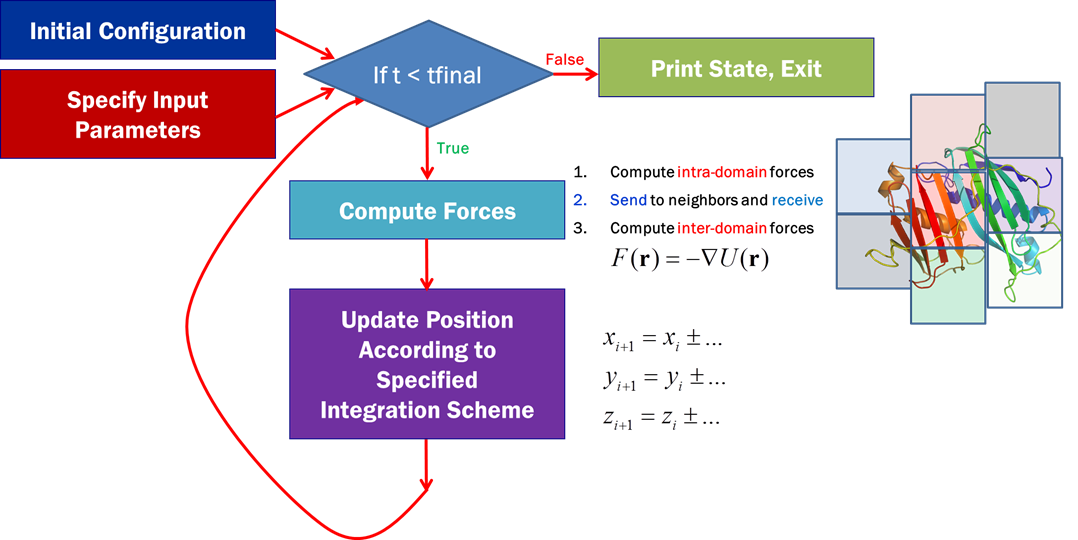
\includegraphics[width=0.49\textwidth]{workflow.png}
	\end{center}
\vspace{-20pt}
\caption{Schematic of typical workflow in a molecular dynamics simulation.}
\vspace{-10pt}
\label{fig: workflow}
\end{wrapfigure}

\begin{enumerate}
    \item Initialize positions and choose a timestep, $dt$
    \item Calculate the forces $\overrightarrow{F} =  -\nabla V (\overrightarrow{r}) $
    \item Numerically integrate to calculate the displacement over $dt$, using the relationships $\overrightarrow{F}=m\overrightarrow{a}$, $\overrightarrow{a} = \frac{\overrightarrow{dv}}{dt}$, and $\overrightarrow{v} = \frac{\overrightarrow{dr}}{dt}$
    \item Update positions and time
    \item Repeat from step 2 until final time
\end{enumerate}

Different potential functions can be used to describe the system at different levels of accuracy, and many forms have been fit to reflect experimental results.
%
These functions typically try to capture van der Waals interactions due to coupling of electron clouds, but can also incorporate additional effects, such as long range charge-charge interactions and solvation interactions (Debye screening effects).
%
Our project provides an easily extensible interface so that the future user can incorporate additional interactions.

For numerical stability, the timestep $dt$ is typically on the order of a femtosecond in ``real" units.  In reduced units, which is what we work in, this is usually about 0.001-0.005.
%
The longest simulations reported for macromolecules such as proteins are on the millisecond timescale, but such lengthy simulations can require specialized supercomputing hardware such as GPUs.
%
At each step, the evaluation of the potential energy and forces can be parallelized, which is the primary reason MD has been so successful on large computer clusters.
%
There are many different numerical integration algorithms that have been developed, each with a slightly different purpose and numerical stability.
%
In this project, we implemented the Verlet integrator (NVE ensemble) and the Andersen thermostat (NVT ensemble), which uses the Velocity Verlet algorithm.
%
Both of these integration schemes were developed specifically for molecular dynamics.

Several existing MD packages, such as HOOMD, LAMMPS, GROMACS, and NAMD, incorporate such ensembles. Members of our group use some of these codes in every day research, but we are not intimately familiar with their internal structure. Therefore, it was a prudent exercise to develop our own codebase with a well-written interface that we can each extend for our custom applications.

\subsection{Verlet integrator}
The Verlet integrator is designed to maintain constant number of particles ($N$), volume ($V$), and energy ($E$) over the course of a simulation.
%
This NVE ensemble is known in thermodynamics as the {\em microcanonical ensemble}.
% 
Such a system is closed and isolated with an equilibrium state characterized by maximum entropy.

The Verlet integrator equations are obtained by expanding  taylor series for the position of an atom forward and backward in time, then summing the two to cancel out terms.. The results is
$$ \overrightarrow{r}(t + \Delta t) = 2 \overrightarrow{r}(t) - \overrightarrow{r}(t- \Delta t) + \frac{\overrightarrow{F}(t) \Delta t ^2}{m}$$

$$ \overrightarrow{v}(t + \Delta t) = \frac{\overrightarrow{r}(t + \Delta t) - \overrightarrow{r}(t)} {\Delta t} $$

\subsection{Andersen thermostat}
The Andersen thermostat is designed to maintain constant number of particles ($N$), volume ($V$), and temperature ($T$) over the course of a simulation.
%
This NVT ensemble is known in thermodynamics as the {\em canonical ensemble}.
%
This scheme is setup in a way such that the system is coupled with an external heat bath that is maintained at a setpoint.
%
Its equilibrium is characterized by the minimum Helmholtz free energy, and energy is not conserved in the NVT ensemble.
%
The kinetic temperature is given by the equipartition theorem.

$$\frac{3}{2} N k_{B} T = \sum_{i}^{N_{particles}} \frac{1}{2} m_{i} \overrightarrow{v{i}}^{2} $$

In this description, the temperature setpoint specified by a user is denoted as $T_{bath}$. The system temperature is denoted as $T_{instant}$.
In the Andersen thermostat, the Velocity Verlet algorithm is used for integration of the equations of motion.

$$\overrightarrow{r}(t + \Delta t) = \overrightarrow{r}(t) + \overrightarrow{v}(t)\Delta t + \frac{\overrightarrow{f}(t)}{2m} \Delta t ^{2}$$

$$\overrightarrow{v}(t+\Delta t) = \overrightarrow{v}(t) + \frac{\overrightarrow{f}(t+\Delta t) + \overrightarrow{f}(t)}{2m}\Delta t$$

The velocity update must be done in a two-step fashion as it depends on the forces at time $t$ and $t+\Delta t$.  In the first part, the forces are calculated between all of the particles. Then, knowing the velocities and forces at time t, we update $\overrightarrow{r}(t)$ and determine

$$\overrightarrow{v'}(t) = \overrightarrow{v}(t) + \frac{\overrightarrow{f}(t)}{2m}\Delta t$$

Then, the force is calculated again after the positions are updated to obtain the velocities at $t + \Delta t$.

$$\overrightarrow{v}(t+\Delta t) = \overrightarrow{v'}(t) + \frac{\overrightarrow{f}(t+\Delta t)}{2m}\Delta t$$

To maintain a constant temperature, the velocities of certain particles interacting with the heat bath (chosen stochastically) are modified from the above scheme. A Gaussian distribution of velocities with a mean of zero and variance $\sigma^{2} = T_{bath}$ must be constructed, denoted as $Gauss(0,\sigma^{2})$. Then, for each particle, a uniformly distributed random number between zero and one is calculated. If this number is less than the interaction parameter $\nu$ multiplied by the timestep $dt$, then the velocities of that particle are updated as

$$ v(i) = Gauss(0,\sigma^{2}) $$

The parameter $\nu$ is the ``collision frequency" which reflects how often a particle from the theoretical heat bath collides with a particle in the simulation and exchanges momentum, thus  conserving temperature stochastically.  The above algorithm proceeds until a pre-specified number of steps has completed.

\section{Code Goals and Structure}
Our code was written with the goals of generalizability and efficiency.
%
Namely we aim to produce a molecular dynamics codebase that can perform simulations
\begin{enumerate}
    \item Using different ensembles
    \item Using an arbitrary number of particles
    \item With an arbitrary system size
    \item Using arbitrary potentials
    \item Parallelized using MPI for use with CPU clusters
\end{enumerate}
%
Our code is written as a mixture of C and C++, and utilizes many object-oriented features.
%
C++ was chosen because of its excellent memory management and object oriented convenience.
%
However, we found that most C features were more convenient when working with MPI (such as the MPI\_Atom structure), and thus the code is a mixture of the two sister languages.
%
Design decisions were constantly assessed for style, convenience, and for ease of understanding.
The code is primarily optimized for small to medium-sized systems, as larger systems would require features that would take much longer to develop than that allowed for in this project (such as neighbor lists, etc.).
In terms of ``make vs. buy", our project is 99.9\% make. That is, the only components of the approximately 4000 lines of code we produced that were not written by our group were BOOST, MPI, and Googletests.
%
The modular class structure allows for a general coding framework, so that users can easily define their own integrators, pair potentials, and bond types in the future.  The ease of this was tested ad hoc by rotating responsibilities in the group for different portions of the code to ensure that it was easy to read and pick up with little to no prior knowledge.
%
We have defined various classes for the different parts of our MD simulation.
%
\begin{enumerate}
\item Atom: This is a C-style structure rather than a C++ class. This structure is passed between processors when the code is run in parallel.
\item Integrator: The integrator class is an abstract base class. It defines the implementation structure for integrators. We have provided two integrators (Verlet and Andersen), but our code can easily be extended to other integration schemes.
\item Interaction: The interaction class is an abstract base class. It defines the interaction between two atoms, including a function pointer to different interaction potentials. We have implemented a shifted Lennard-Jones potential, a harmonic bond potential, and the finitely extensible nonlinear elastic (fene) bond potential. 
\item System: The system class stores the majority of the information for the simulation including the box size, a list of atoms, and the interactions between atoms (stored as a matrix of Interaction classes). When the code is run in parallel, each processor contains a system object that contains the atoms owned by that processor.
\end{enumerate}

The files ``read\_interaction.cpp'' and ``read\_xml.cpp'' handle file I/O and initialization of these System classes.
%

The flow of our code is as follows:
\begin{enumerate}
\item The code reads in the starting configuration from the user-supplied xml file, and the relevant energy parameters from the user-supplied energy file. Atoms are read from the xml file and assigned to the correct processor. See initialize.cpp for more details.
\item A System object is instantiated for each processor containing the relevant parameters read from the files.
\item An integrator is set.
\item The forces on each atom are calculated using the ``minimum image" distance between atoms that exist on the same processor.  This refers to the conventional use of the smallest distance, $r$, between periodic images of atoms in the interparticle potential energy functions.
\item When the code is run in parallel, the ``ghost'' atoms near the edges of each processor domain are passed to the relevant neighboring processors, and the forces between these ghost atoms and the atoms ``owned" by the processor are calculated.
\item The atomic positions are updated via the ``step()'' function for the instantiated integrator.
\item Any atoms that have moved outside of the processor domain are passed to the new processor that ``owns" them.
\end{enumerate}
Steps 4-8 are repeated for each timestep.
%
At each time step, the configuration of the system is output to an animation file (.xyz).  This file is printed to after each step in the simulation which can be slow (on many processors) due to communication losses, but also produces high quality movies.
%
This file can be read by VMD, a molecular visualization package, to produce such a movie. 

\subsection{Input and Output}
Initial configurations are specified through xml files.  This is documented by example below.  To be more general and work with xml formats of other programs like HOOMD, our parser can read data blocks in any order by invoking the rewind() function and scanning the file for keywords that define the start of a block.  This file is read in ``cascade" by multiple processors, that is, when more that one processor is used, it is read sequentially by each processor which signals the next one in line once it is finished.  The reasons for this are discussed further in Sec.~\ref{sec: details}.  We used the Boost C++ library to allow for discrepancies in the xml file (such as extra white spaces, tabs, etc.) to be as flexible as possible (cf. read\_xml.cpp)
%
\begin{verbatim}
<?xml version="1.0" encoding="UTF-8"?>
<hoomd_xml version="1.4">
<configuration time_step="0" dimensions="3" natoms="2" >
<box lx="10" ly="10" lz="10"/>
<position num=�2">
6.22 5 5
3.78 5 5
</position>
<velocity num="2">
0 0 0
0 0 0
</velocity>
<mass num="2">
1
1
</mass>
<diameter num="2">
1
1
</diameter>
<type num="2">
A
A
</type>
<bond num=�1">
feneA 0 1
</bond>
</configuration>
</hoomd_xml>
\end{verbatim}

The energy file contains the parameters for each interaction type in the xml file, as shown below. These files are parsed by reading a keyword from the beginning of each line.  These can be either ``PPOT" for a pair potential, or ``BOND" for a bonding potential.  This is followed by the name of the ``types" involved in the interaction, which for PPOT is two atom types, while simply a name for BOND.  What follows is specific to the interaction type.  Refer to the factory function get\_fn() in read\_interaction.cpp for a list of the expected parameters and order they are to be specified in.  The parameters for a shifted Lennard-Jones interaction are $\epsilon$, $\sigma$, $\Delta$, $U_{shift}$, and $r_{cut}$.  It should be noted that good parameters are hard to come by in MD and the examples we provide below and on the repository (cf. LJ.energy) are stable, well-researched values.  Deviation from these parameters can easily lead to (validly) poor simulations. 

\begin{verbatim}
PPOT A A slj 1.0 1.0 0.0 0.0 2.4
PPOT A B slj 1.0 1.0 0.0 0.0 2.4
PPOT B B slj 1.0 1.0 0.0 0.0 2.4
BOND feneA fene 1.0 1.0 0.0 30.0 2.4
\end{verbatim}

This file is read in a cascade similar to the input xml file. The energy file parser's advantages include a ``factory-style'' workflow for generating the interaction matrix in the System objects, which allows for easy future expansion.  We again use Boost to help parse the file (cf. read\_interaction.cpp).
The shifted Lennard-Jones potential corresponding to the energy parameters listed above is given by
$$
U(r) = 4\epsilon \left( \left( \frac{\sigma}{r-\Delta} \right)^{12} - \left( \frac{\sigma}{r-\Delta} \right)^{6} \right) + U_{shift} ,   r - \Delta < r_{cut} $$
and the Finitely Extensible Nonlinear Elastic Model bond potential (FENE bond) can be written as
$$U(r) = -\frac{1}{2} k r_{0}^{2} \text{ln} \left(1 - \left( \frac{r-\Delta}{r_{0}} \right)^{2} \right) + U_{WCA}$$

The force on a particle is given by 
$$ F_{i} = - \frac{\partial U}{\partial r} \frac{\partial r}{\partial x_{i}} = - \frac{\partial U}{\partial r} \frac{x_{i}}{r}$$

Refer to interaction.cpp for more details on all the different interactions.  

\subsection{Domain decomposition}
In the final version of our code, we utilize a one-dimensional domain decomposition, where the simulation box is decomposed into vertical slabs.
%
Each vertical slab and the atoms it contains are assigned to a processor, and atoms are passed between processors as needed using MPI as the system evolves in time.  The width of each domain must be at least the maximum range of the interaction cutoff.  That is, above some distance, $r_{cut}$, interactions are set to 0 to make the simulation feasible (set in energy file).  This can be different for each interaction present in a system, but we are only concerned with the maximum.  We have prescribed that only nearest domains should interact with one another, therefore an atom in say, domain 1, cannot be allowed to interact with an atom in domain 3.  Therefore the minimum domain size is $r_{cut,max}$ (see read\_interaction.cpp) which places a maximum on the number of processors that can be used for a simulation.  For instance, for a system with a cubic box having sides of length 10, with particles interacting through a Lennard-Jones potential cutoff at 2.5, the maximum number of processors allowed is 4 (this is commonly the case found in the following examples and in those provided in the repository).  Any attempt to use more than this is checked by the code and alerts the user to the error before exiting gracefully.
\par
	However, we began our project by attempting a three-dimensional domain decomposition.  Although we could not get this algorithm completely debugged by the end of the project, we include information on the structure and implementation here since it comprised a large portion of our efforts. The 3-D domain decomposition attempts to spatially split the simulation box into a number of identical domains based on the number of processors available. Each processor will then be responsible for one domain. Parallelization will be most efficient if each processor has approximately the same load.  If we assume that the particles are uniformly distributed in the simulation box, then the most efficient way to partition the system is one in which the individual domains are as cubic as possible.
%
This is what the 3-D domain decomposition algorithm attempts to do. Note: The 3-D domain decomposition assumes that the simulation box is a rectangular parallelepiped
with one corner positioned at (0,0,0). The algorithm is as follows:
\begin{enumerate}
\item Generate the prime factorization of the number of processors available (e.g. $36 = 2 \times 2 \times 3 \times 3$).
\item Generate a set of 3 numbers by combining the factors in different ways such that the product
is still the number of processors available (e.g. for the case of 36 processors, possible sets are

$\{2,3,6\}, \{3,2,6\}, \{1,4,9\}, \{2, 1, 18\}$, etc.).
\item Divide the simulation box into domains by dividing the $x$, $y$, $z$ directions respectively into a
number of parts based on the 3 numbers in one of the sets generated in step 2. (See Fig. \ref{fig: ddecomp} for an
example)
\item Check how cubic the domains are by evaluating $diff = (d_1-d_2)^2+(d_2-d_3)^2+(d_3-d_1)^2$ ; where $d_1$, $d_2$, $d_3$
are the $x$, $y$, $z$ dimensions of a domain (since all the domains are the same size and shape).
\item Repeat steps 3-4 for all the sets generated in step 2 while keeping track of the set that resulted
in the smallest value of diff.
\item Divide the simulation box into domains based on the set which generated the smallest value of diff.
\item Assign the domains to processors by stepping through each domain in the $x$-direction from
lowest to highest, then in $y$, and then in $z$. (See Fig. \ref{fig: ddecomp} for an example)
\end{enumerate}

\begin{wrapfigure}{l}{0.5\textwidth}
\vspace{-30pt}
	\begin{center}	 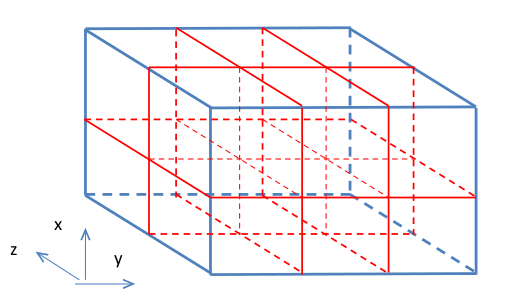
\includegraphics[width=0.49\textwidth]{ddecomp.jpg}
	\end{center}
\vspace{-20pt}
\caption{An example of the domain decomposition. The set in use is $\{2,3,2\}$ (see step 3 of the algorithm).}
\vspace{-10pt}
\label{fig: ddecomp}
\end{wrapfigure}

The code implements steps 2-4 through the recursive function gen\_sets in domain\_decomp.cpp.
The function init\_domain\_decomp in domain\_decomp.cpp starts the process from step 1 through 6
calling gen\_sets along the way.

\section{Validation}

We have verified the accuracy of our simulations by comparing our results to LAMMPS, a commercial/academic molecular dynamics software package. Energy (or temperature, depending on the ensemble) as a function of time matches our results identically.  Additionally, the radial distribution function $g(r)$ was calculated over the course of a 1000 timestep simulation for a 1000 particle system. The initial coordinates and velocities of this system was input to LAMMPS and into our NVE code independently and simulated.  The comparison is shown in Fig.~\ref{fig: validate}.  As you can see, these results are identical.

\begin{figure}[htb]
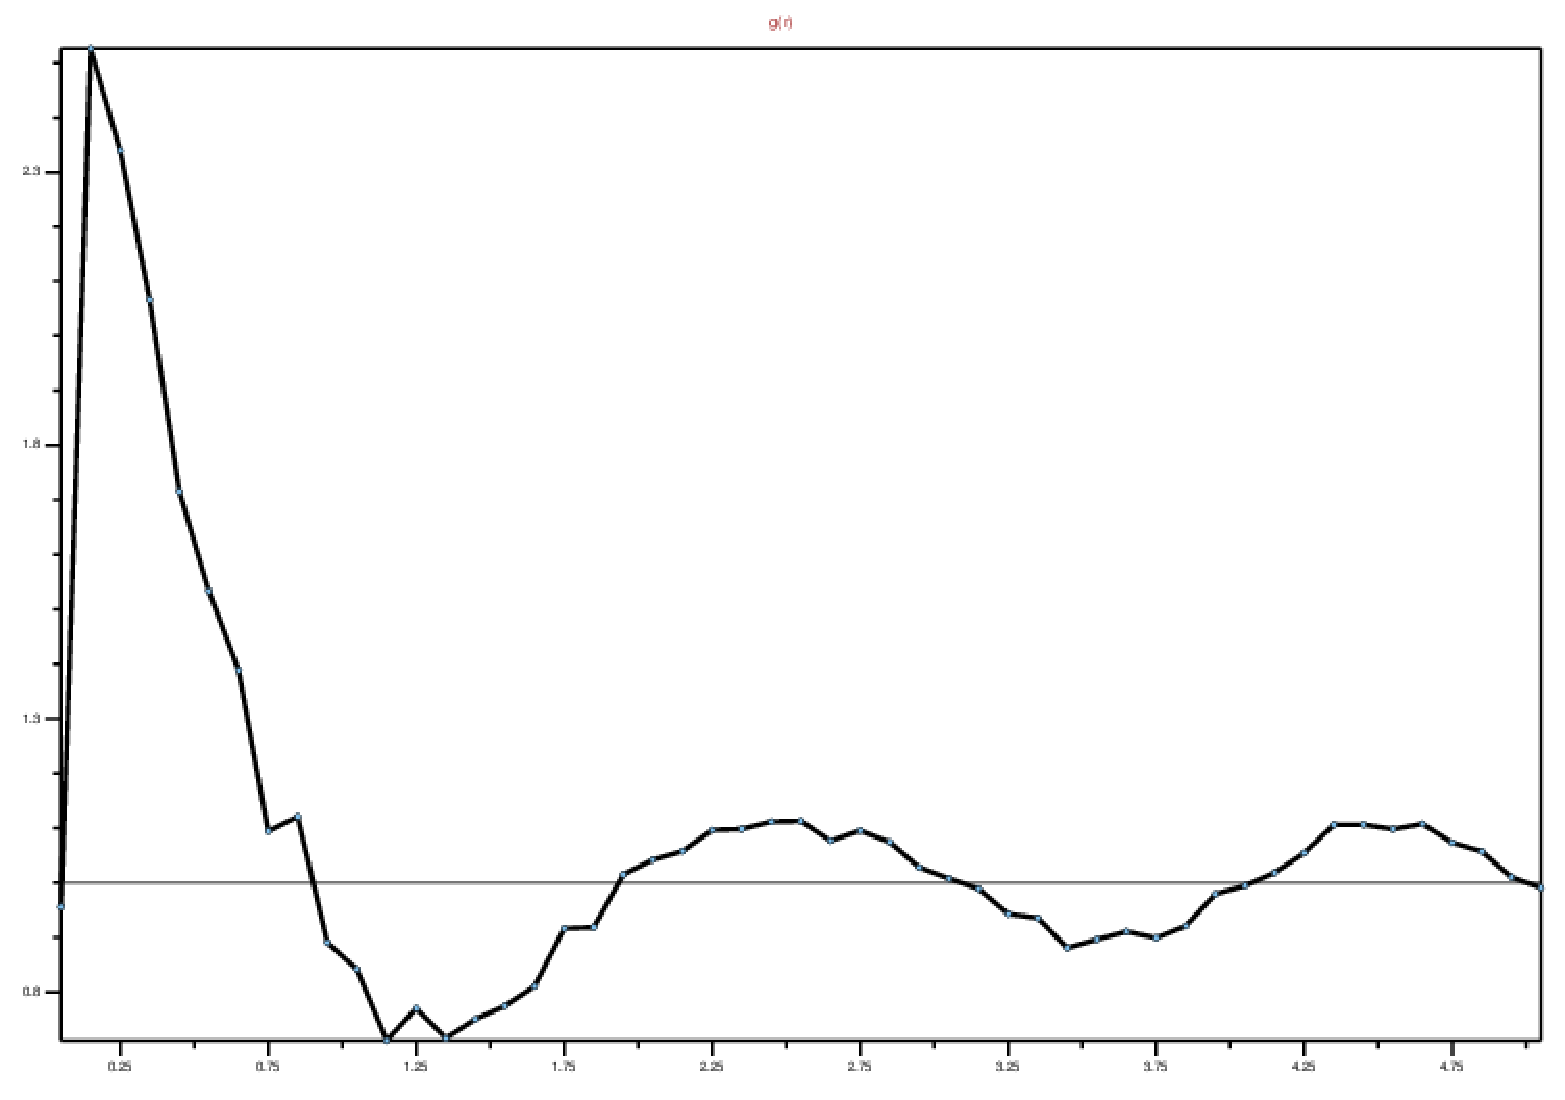
\includegraphics[width=0.5\textwidth]{gr_1000_cbemd.pdf}
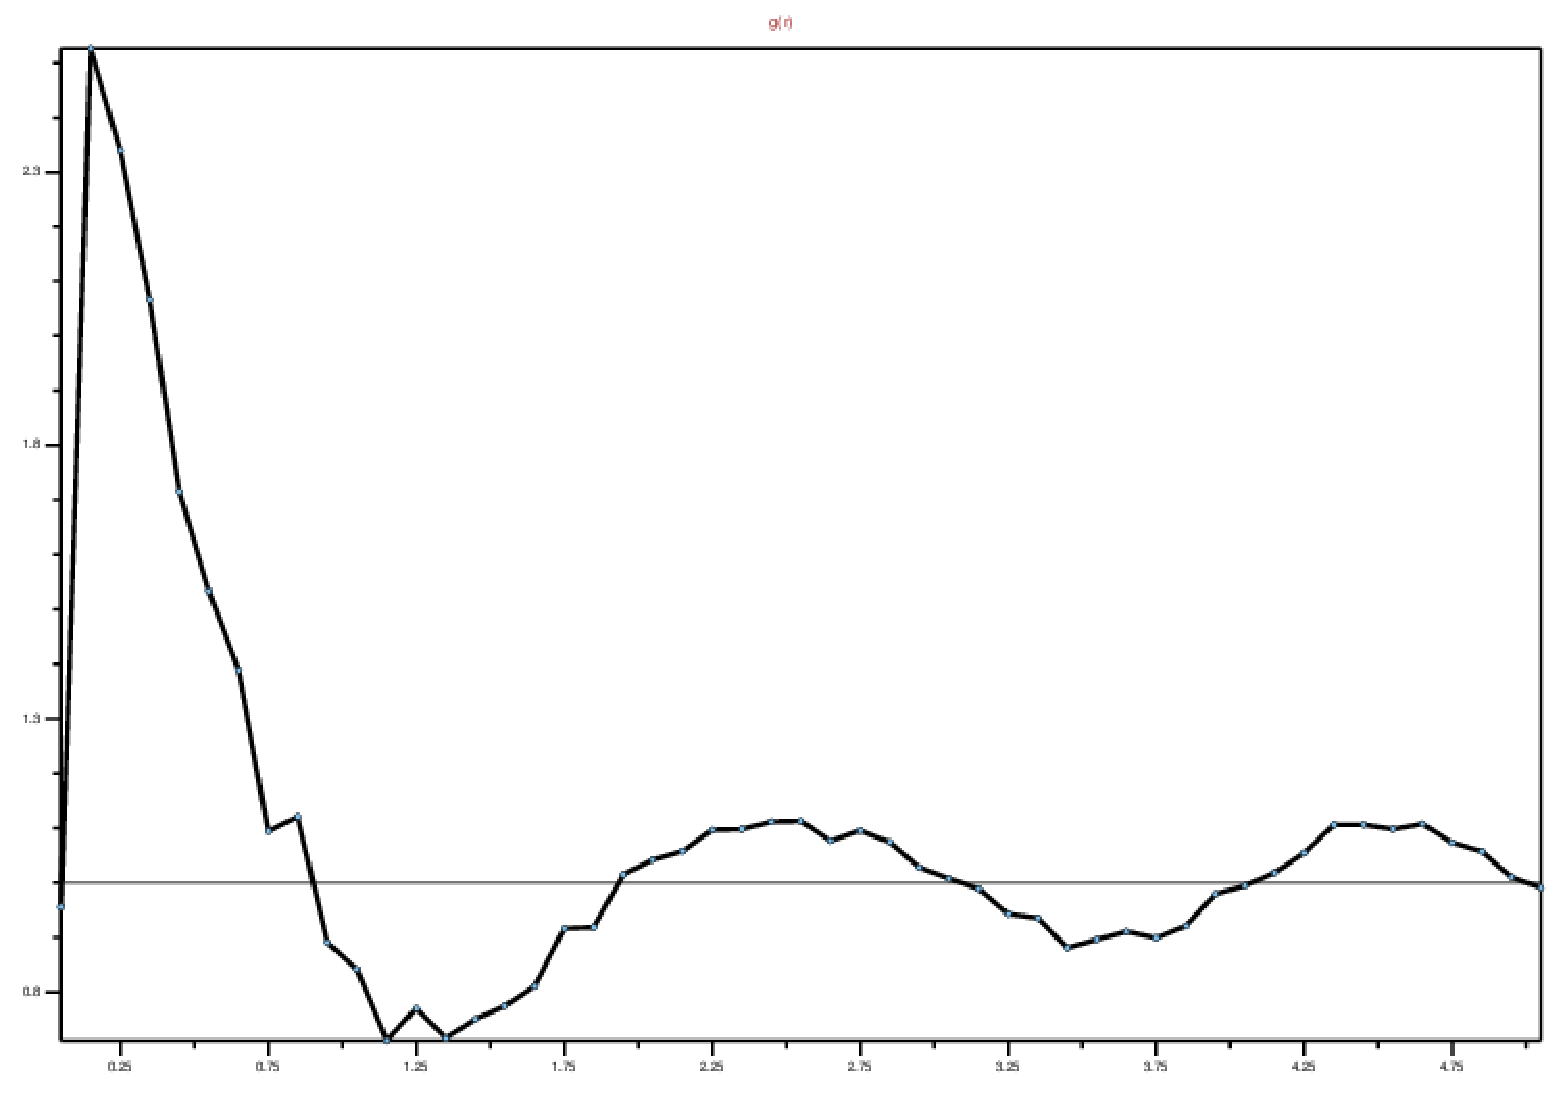
\includegraphics[width=0.5\textwidth]{gr_1000_lammps.pdf}
\caption{Comparison of the radial distribution function $g(r)$ for our code (left) and LAMMPS (right) for a 1000 atom system of identical Lennard Jones particles at $t=1000$ timesteps. The ordinate is the radial distribution function, $g(r)$, and the abscissa is the separation distance between particle centers, $r$.}
\label{fig: validate}
\end{figure}

\begin{figure}
	\begin{center}	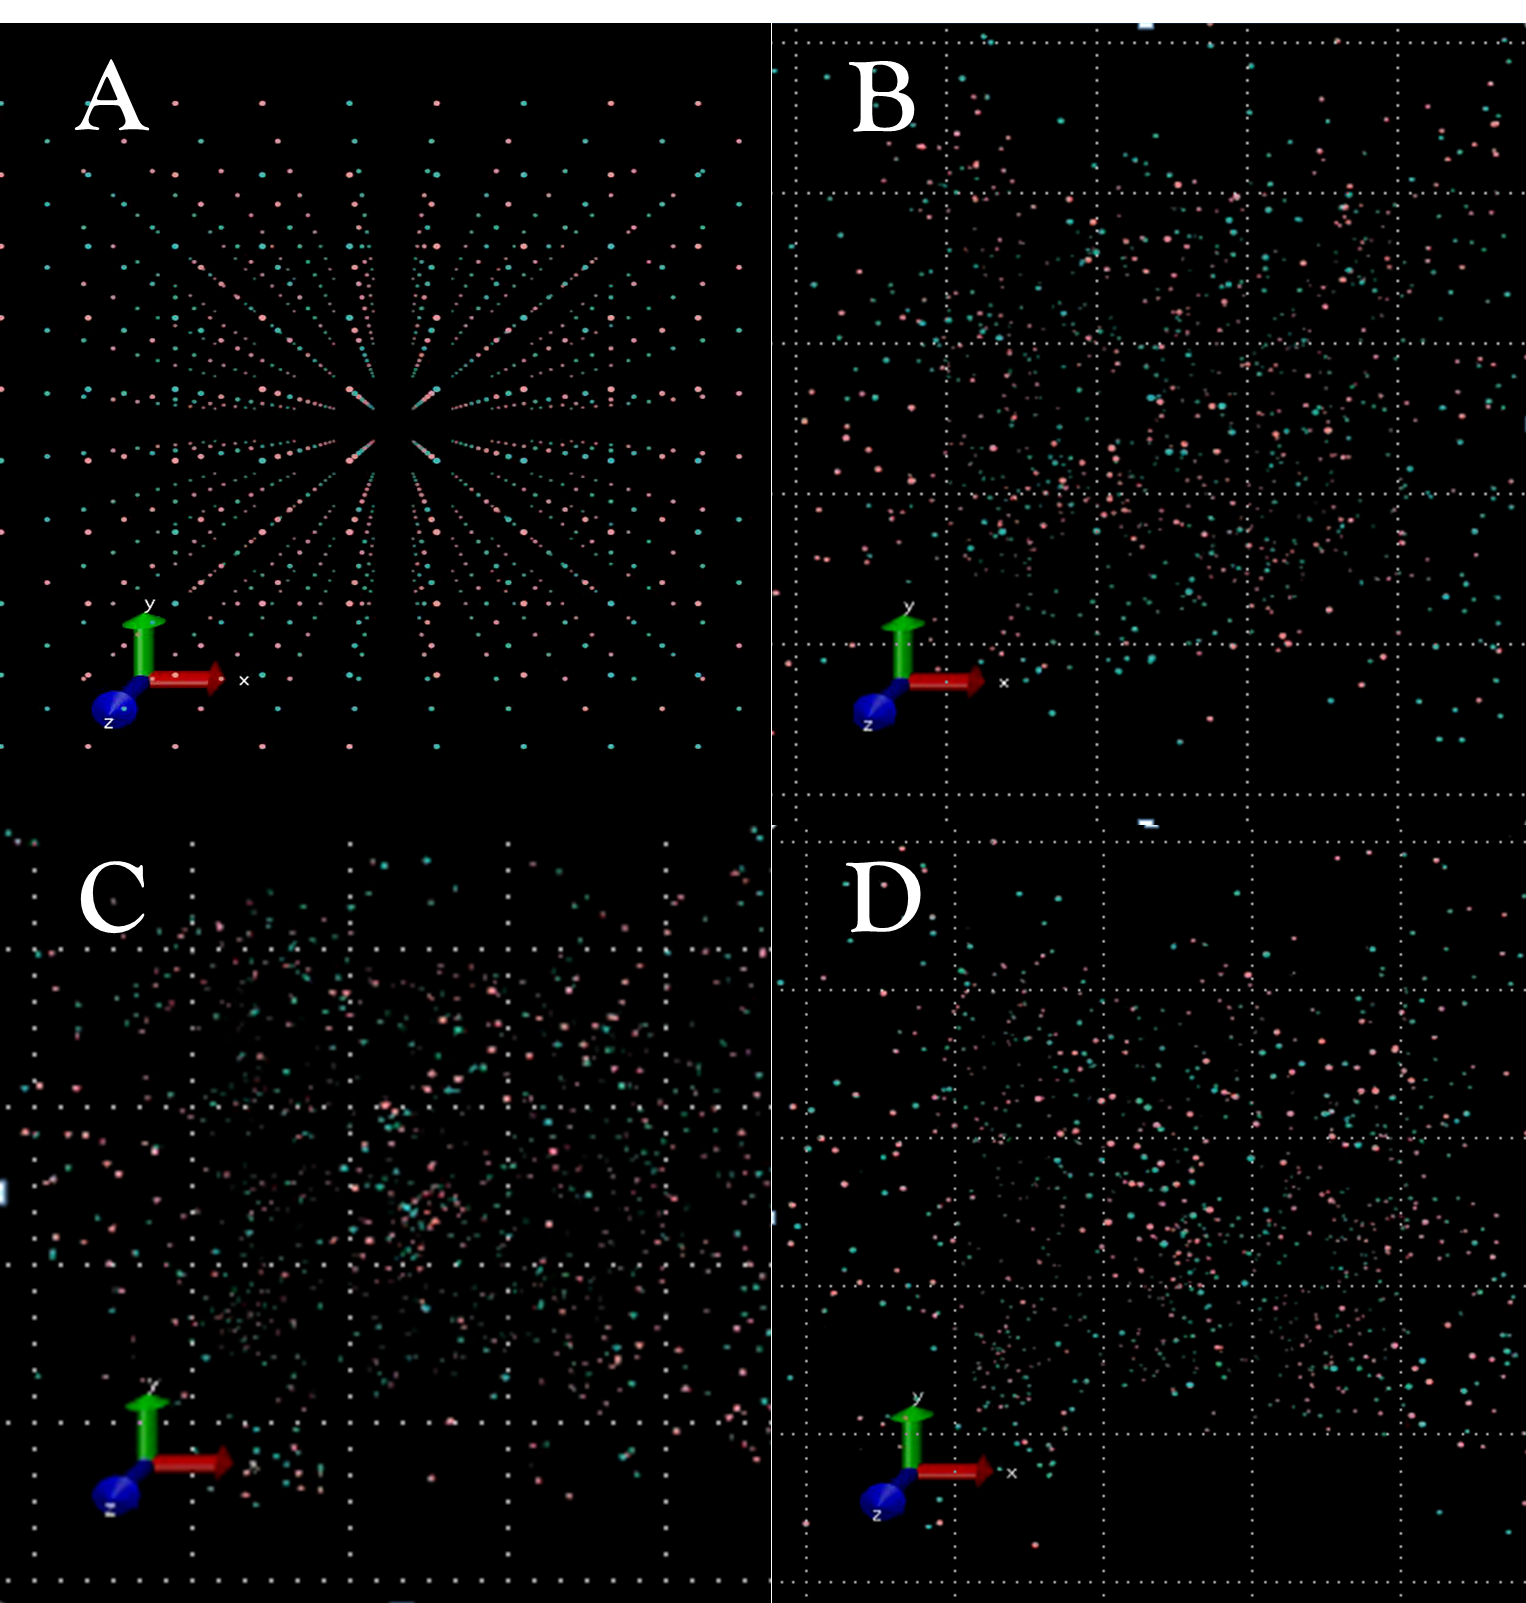
\includegraphics[width=0.5\textwidth]{snapshots.png}
	\end{center}
	\caption{The evolution of a binary system of 1000 Lennard-Jones particles over time.}
\end{figure}


%The radial distribution function is a very important metric that describes the probability of finding two particles at a distance $r$ from each other. 
%From $g(r)$, its possible to derive macroscopic thermodynamic values such as the potential energy and pressure of a system. \textit{It is evident in ~\ref{fig:validate} that the $g(\overrightarrow{r})$ produced by CBEMD is identical to that produced by LAMMPS, validating the accuracy of our program.}

\subsection{Testing}
Testing was performed using googletests to test individual key components of CBEMD. 
%
However, the ultimate test is the exact agreement between results generated by CBEMD and that produced by the commercial package LAMMPS as shown previously.
%
Nevertheless, 21 tests were written to verify components of domain decomposition, calculation of the harmonic bond, fene bond, shifted Lennard-Jones potentials, file I/O, etc. for both single and multiple processors.  These tests are located in test\_all.cpp and can be made with MakefileTests (see README for more details).
\begin{figure}[htb]
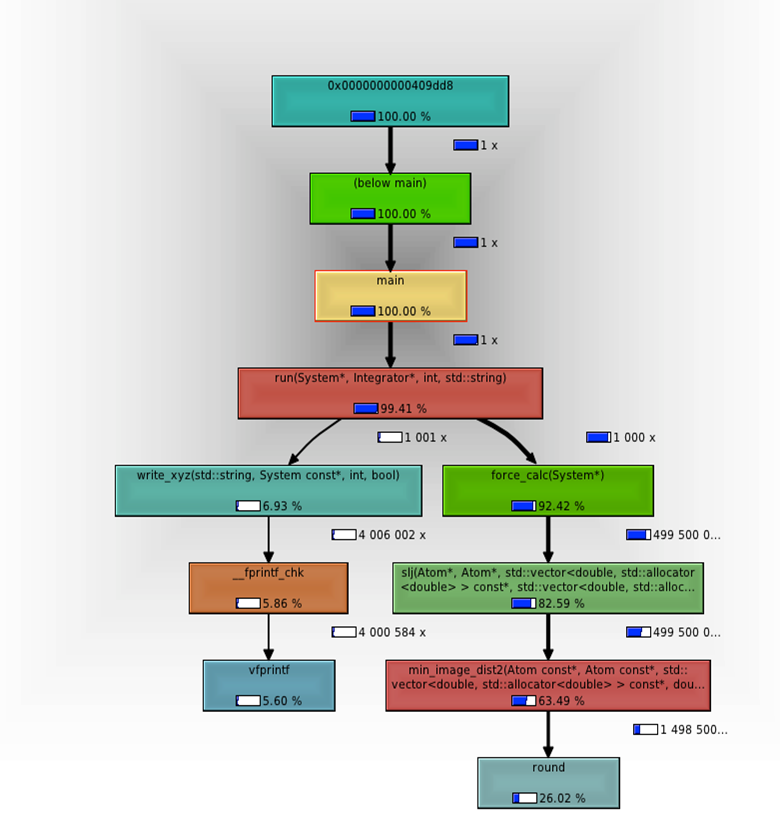
\includegraphics[width=0.5\textwidth]{serial.png}
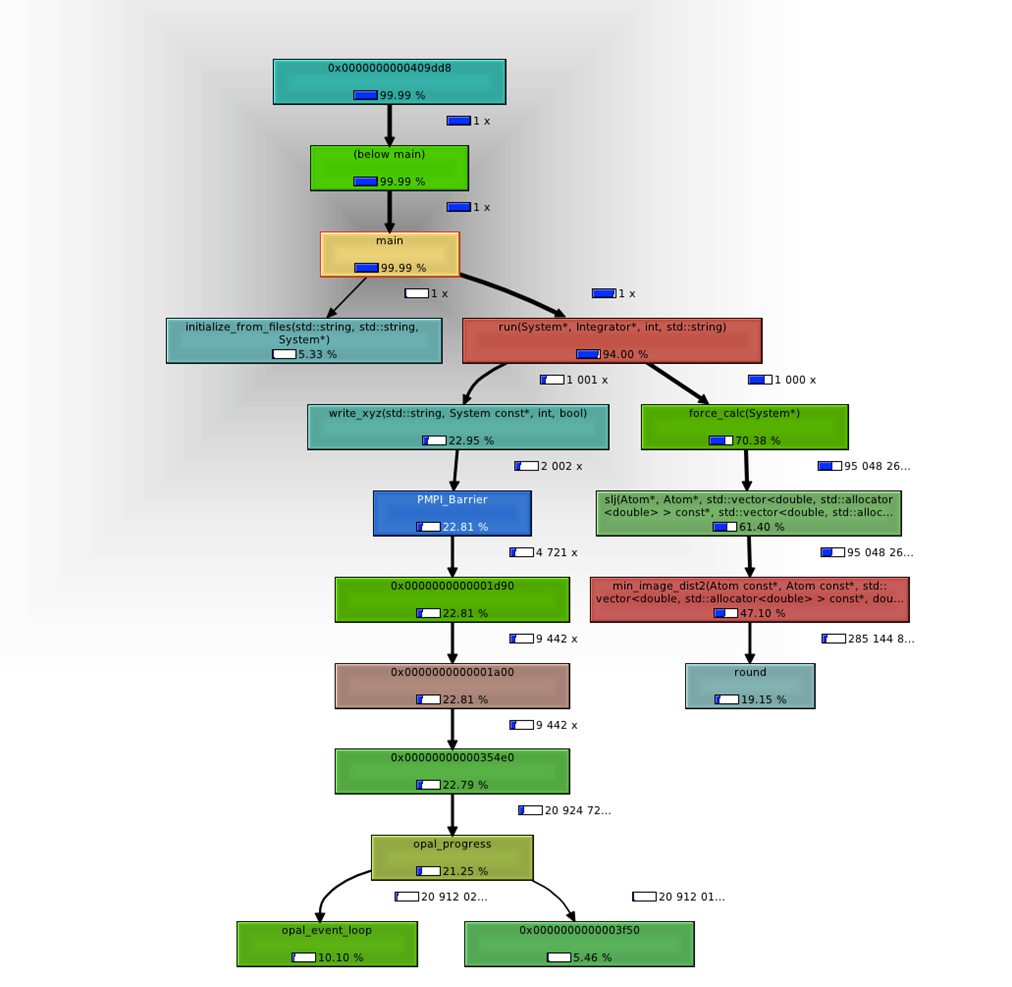
\includegraphics[width=0.5\textwidth]{mpi4procs.png}
\caption{The results from profiling using Kcachegrind while running the code in serial (left) and in parallel on four processors (right).}
\label{fig: profiling}
\end{figure}

\section{Comments on Specifics \label{sec: details}}
\par
	It is impossible to enumerate all cases of the subtle design decisions made over the course of this project, but here we discuss a few.  There are a number of features in the code we have not discussed previously that deserve mention as they were the source of some debate and represent significant work.  Many instances are marked improvements to the interface between the user and the code that are not found in many publicly available production codes.  
	\par
	For example, the nature of many such codes (due to legacy issues from the days of Fortran) require the user to numerically order bond, atom, and interaction types.  Instead, our code uses maps to identify user-defined names for such types which can be much more understandable.  For instance, the user may specify an atom type as ``Hydrogen" or ``myatom1" rather than using indices like 0 and 1 which are required in LAMMPS.  This makes the extraction of information in the midst of a simulation about specific interactions much easier.  The user can extract all information about a certain atom or bond type through System member functions like bond\_type() or atom\_type() which return the internal index of these types, which are hidden from the user to avoid confusion and/or mistakes in analysis.
	\par
	Second, functions usually return an error code rather than using the C++ throw/catch syntax.  Although this is used in select places because an error must be caught at a higher level, in most instances we found that error flags were more useful.  This is bit specific for our intended future applications which include wrapping in python, either through SWIG or simply by calling the command line through the ``os" module in python.  The latter can catch output flags automatically and is already implemented nicely.  As a result we found that for the most part, using flags allowed us to interface with python more conveniently.
	\par
	Third, when using MPI we load information for all processors by reading in a ``cascade"; that is, a processors reads and parses and xml and energy file, then signals the next processor in line to do this once it is finished.  This is a reasonably efficient scheme for small numbers of processors (which was our intended target for small systems).  Although it is possible to parse the information all on one processor then use MPI calls to communicate the data, a majority of the information in these file is necessary for the initialization of certain matrices (such as System.interact) for \emph{every} domain's System object.  As a result, it was much simpler to have each processor just read the files, rather than continuously passing around nearly all the information anyway.
	\par
	Additionally, in keeping with our intended target of optimizing the code for small systems, we implemented a matrix of interactions (see System.interact).  The reason is that, by convention, when two atoms interact through  bonding potential they do not interaction through anything else.  If all atoms of type ``A" in a system interaction through a certain Lennard-Jones potential, but a select few of them are bonded, this requires substantial effort to check each time a force is calculated if two atoms are involved in a bond, and if so, do a different force calculation.  For medium to small systems, it is much more efficient to simply generate a matrix of interaction classes at the beginning of the simulation that contain function pointers for each pair.  This requires no ``bond-lookup" whatsoever (saving significant time) and is a unique feature of our code.
	\par
	Finally, we gave a significant amount of consideration to the portability of our code.  A major part of this stems from the MPI\_Atom structure.  The way a structure's elements are committed to memory via MPI relies on establishing the proper memory offsets between members.  Certain compilers have been known to have strange padding issues if offsets are not measured explicitly.  As a result, we adopted a ``compiler-safe" scheme in atom.cpp which uses explicit MPI\_Get\_address rather than MPI\_Type\_extent calls to rigorously enumerate these locations in memory (the latter may fail to offset consecutive members properly if abnormal paddings exist).  See comments therein for more details.  Also due to compiler compatibility issues, we have specifically programmed the interactions in interaction.cpp in ways that may seem significantly less readable than the form of their equations may suggest (cf. interaction.cpp).  For instance, taking powers of quantities (cf. Lennard-Jones equation) is done with atomic operations, where division by a quantity is necessary we replace it with a multiplication by a variable whose value is the inverse, etc.  These types of ``improvements" circumvent the use of slow math library functions and perform much faster when compiled with gcc.  Other compilers (like Intel's icc compiler) are intelligent enough to apply these optimization at compile time making this coding practice seemingly obsolete, however, as such compilers are generally not free, we spent significant effort designing code that contains these optimizations manually.  As will be discussed in more detail in Sec.~\ref{sec: optimize}, the end result is a code whose performance is nearly independent of the compiler used.
	
\section{Instructions for using CBEMD}

This project has two driver programs, andersen and verlet; one for each integrator implemented.  They are called from the command line with arguments documented in their respective .cpp files and in the README.  See these files for details and examples on how to use the program properly.

\section{Profiling and Optimization \label{sec: optimize}}
We used gprof to profile our code and highlight the computational bottlenecks (see Fig.~\ref{fig: profiling}).  The majority of the time is spent on the force calculation, with the calculation of the shifted Lennard-Jones (or other) potential and the minimum image distance comprising the majority of the effort.  As mentioned previously, the replacement of math library functions such as pow() and round() also led to significant improvements when possible (Figure~\ref{fig: profiling} illustrates the significant time spent calling round() before we replaced this).
	\par
From the results of our profiling, we focused on optimizing the ``min\_image\_dist2()'' and the potential energy functions.  The ``min\_image\_dist2()'' used the round() function whereas the potential energy functions (such as slj()) employed the pow() function often.  We found that we were able to replace these with while() loops and atomic operations, respectively.

\begin{wrapfigure}{r}{0.5\textwidth}
\vspace{-20pt}
	\begin{center}	 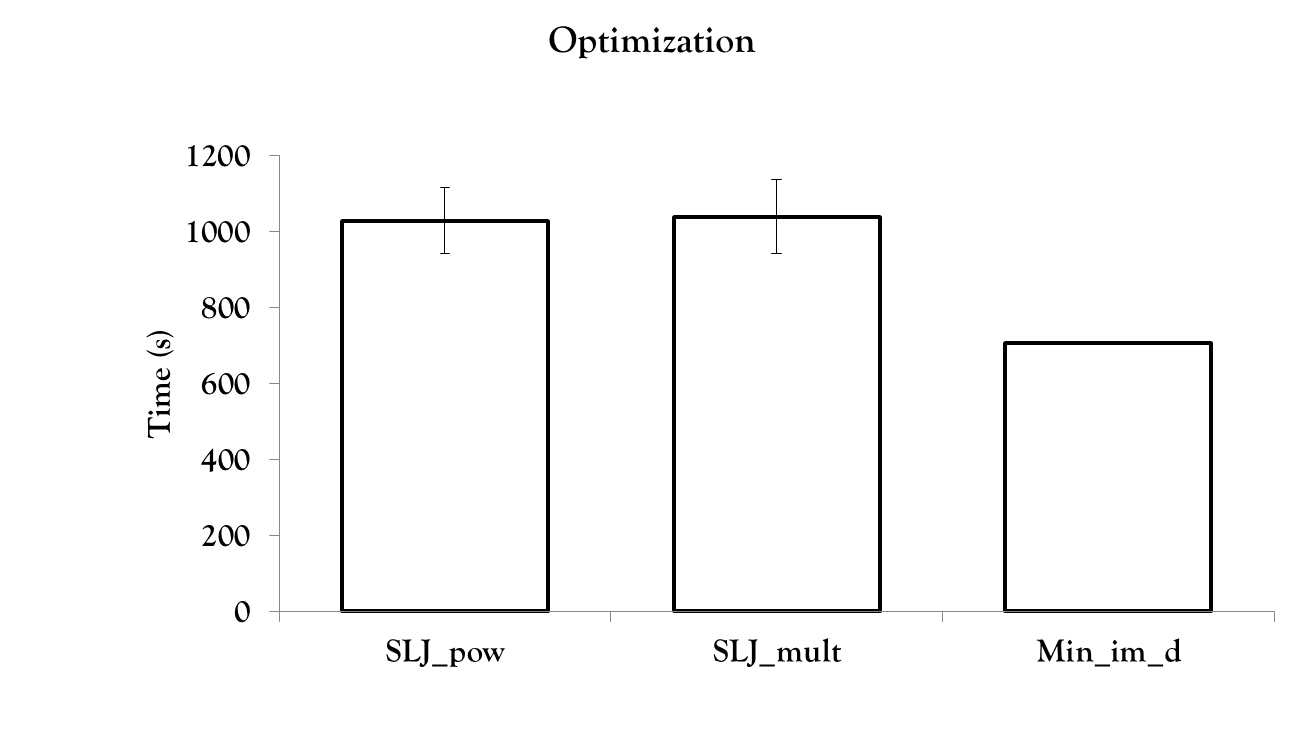
\includegraphics[width=0.49\textwidth]{optimization.png}
	\end{center}
\vspace{-20pt}
\caption{Timings for a system of 1000 Lennard-Jones particles using the pow() function to compute the slj() function (left), atomic operations (middle), and using while() loops to replace the round() math function in min\_image\_dist2() (right).}
\vspace{-10pt}
\label{fig: optimization}
\end{wrapfigure}

The results are shown in Fig.~\ref{fig: optimization}.  The removal of the round() function in the minimum image distance calculation reduced the time from approximately 1000 to 700 seconds, which is a significant reduction.  Conversely, comparing the time where the slj() function used pow() vs atomic operations showed no improvement.   This was initially unexpected, though we eventually uncovered the cause to be the use of the intel compiler, icc, which when using the optimization flag -O3, will automatically convert uses of pow() to atomic multiplications.   As previously mentioned, this is not true for gcc, however, the aforementioned improvements resulted in identical performances for both compilers in the end.

\section{Scaling}
\begin{figure}[h]
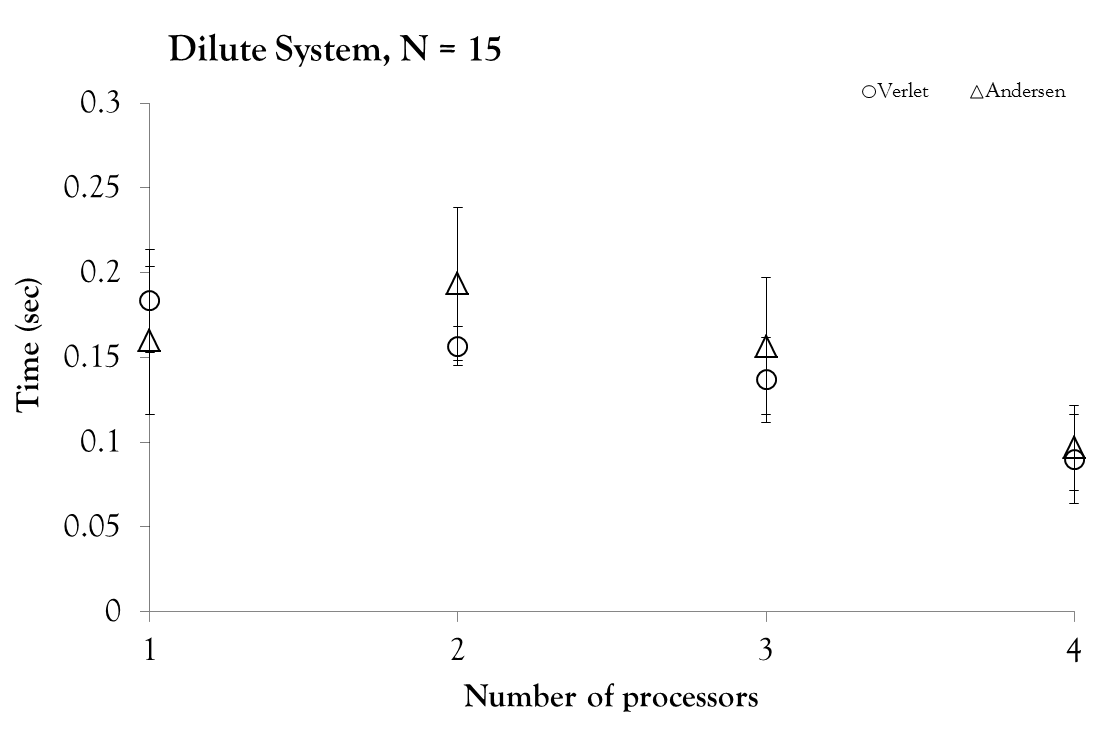
\includegraphics[width=0.5\textwidth]{scalingdilute.png}
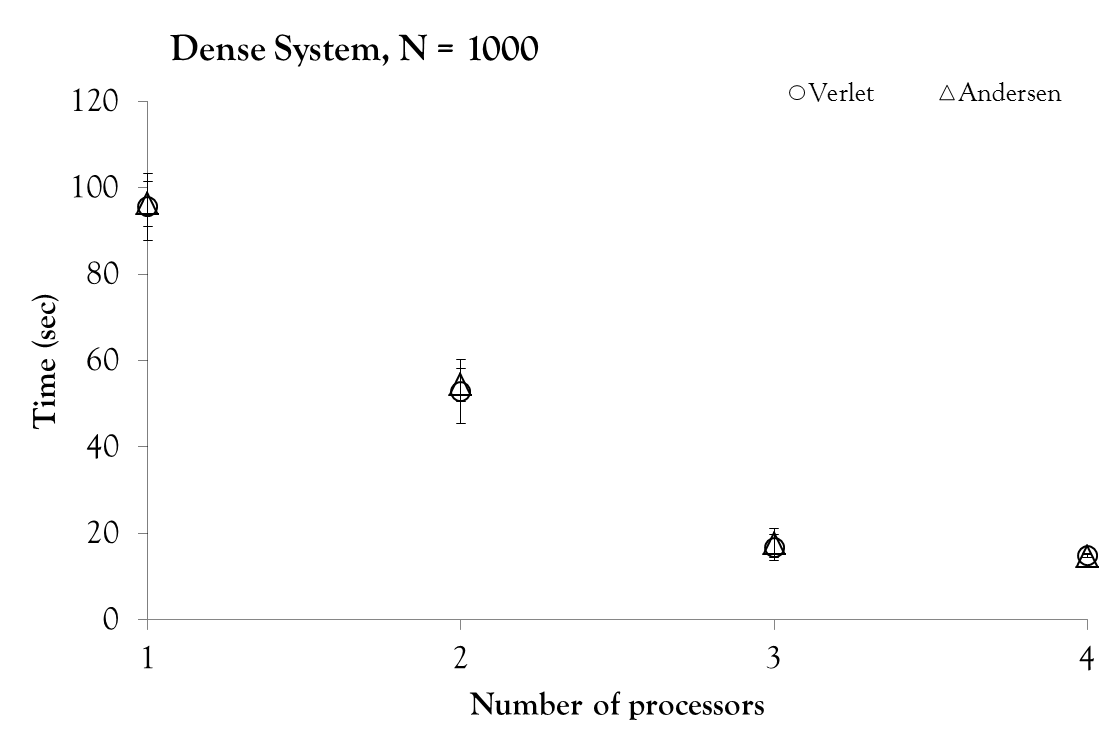
\includegraphics[width=0.5\textwidth]{scalingdense.png}
\caption{Scaling results as a function of number of processors for a dilute system (left) and a dense system (right).}
\label{fig: scalingprocs}
\end{figure}

We looked at how the execution time of our code scaled with the number of processors and with system density.  For a dilute system, there are only marginal gains achieved when increasing the number of processors; because it is so dilute, it is rare that information needs to be passed between processors making the use of additional cores irrelevant. Conversely, for a dense system, there are many instances where information must be passed from processor to processor, so partitioning the calculation across many cores decreases the total time significantly.  In theory, a simulation with twice as many processors should ideally take half as long, suggesting a scaling of $1/n$, where $n$ is the number of processors.  As evidenced by Fig.~\ref{fig: scalingprocs} for the dense system this is recovered quite nicely.
\par
	In the case where we fix the number of processors (in this case, 1), as density increases the simulation time should increase quadratically since interactions are pairwise.   It is evident that the both the Verlet and Andersen integrators scale nearly quadratically with system density, as expected, with only some small communication losses leading to an exponent slightly greater than 2.  This, however, is excellent scaling and on the same order as commercial codes.

\begin{figure}[htb]
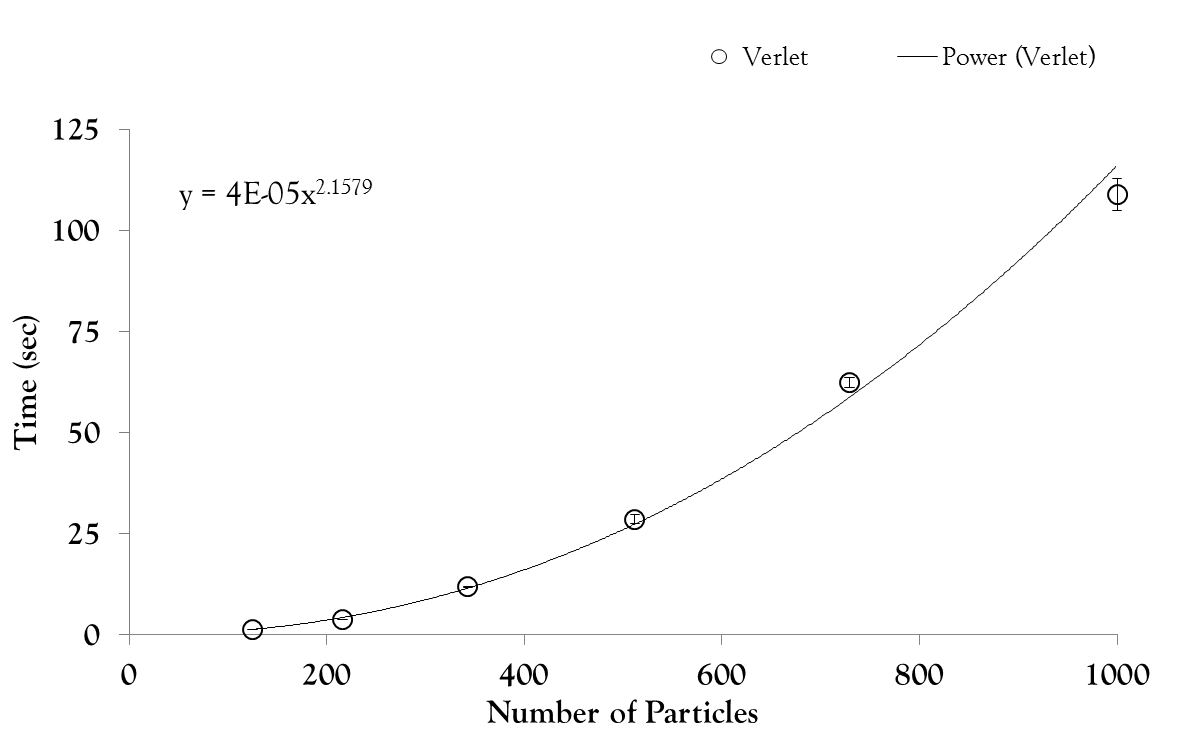
\includegraphics[width=0.5\textwidth]{scalingverlet.png}
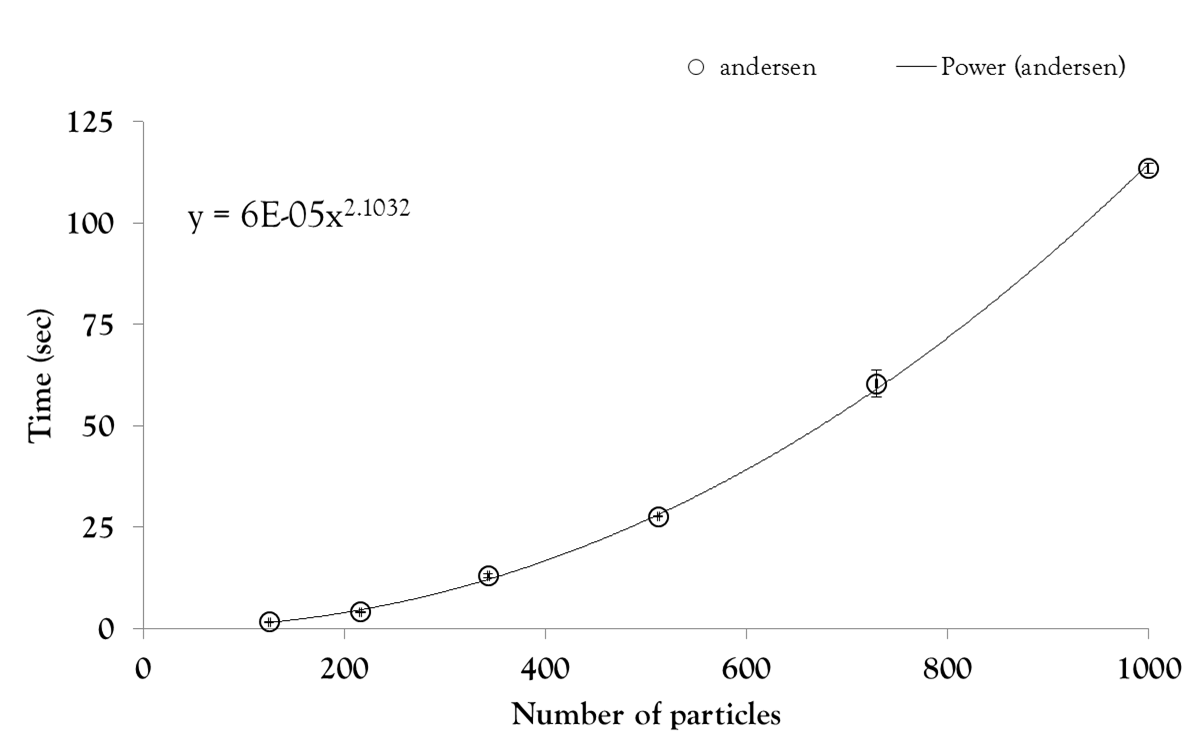
\includegraphics[width=0.5\textwidth]{scalinganderson.png}
\caption{Scaling results for serial integration under the NVE ensemble (Verlet, left) and NVT ensemble (Andersen thermostat, right).}
\label{fig: scaling}
\end{figure}

\section{Documentation}
All documentation of the code was done in Doxygen. A pdf file, refman.pdf (see report/finalreport/ directory), is our reference manual and is included on the repository. In addition, the code comes with a README.md file that contains instructions on how to compile and run the code, as well as how to run the code on the university clusters, with sample PBS scripts and sample run commands.
\section{Conclusion}
In conclusion, we have written a reasonably efficient, portable code that performs molecular dynamics simulations for multiple thermodynamic ensembles in parallel.  It scales reasonably with system size up to an arbitrary number of particles and number of processors, and is easy to expand upon (additional pair or bonding potentials, etc.) because of the effective use of abstract base classes and factory functions.  It outputs files that can be visualized easily with existing software such as VMD, and has been verified with results from publicly available packages such as LAMMPS.
\end{document}
